\chapter{Fundamentos}
\label{cap:fundamentos}

Para melhor exemplificar o funcionamento dos sistema implementado, é pertinente introduzir alguns fundamentos utilizados. 

\section{Enumeração de DNS}

Enumeração de DNS é uma técnica que consiste em obter registros de DNS e seus respectivos valores (geralmente endereços de IP) sem conhecimento prévio. Existem diversas maneiras pelas quais um registro pode ser descoberto, e vale ressaltar que todos esses métodos podem ser utilizados recursivamente nos subdomínios encontrados para uma busca ainda mais completa.
        
        \subsection{Força bruta} São testados diversos nomes comuns  de subdomínios e de serviços conhecidos em um servidor de DNS para verificar se algum deles está disponível no domínio em questão.
        
        \subsection{Web Crawling} Se o domínio principal estiver rodando um servidor HTTP, é possível rodar um \textit{crawler} nele que busca por subdomínios deste mesmo domínio.
        
        \subsection{Search enging scraping} Este método consistem em buscar o domínio principal em um motor de busca existente (como Google ou DuckDuckGo), filtrando através de comandos desses motores de busca para páginas daquele domínio (usando "inurl:example.com", por exemplo).
        
        \subsection{Extração de certificados}: Através deste método, são verificados os valores válidos para subdomínios encontrados nos certificados TLS fornecidos pelos servidores HTTP rodando no domínio principal. Além disso, em alguns casos também é possível pesquisar diretamente em algumas das próprias autoridades certificatórias por possíveis subdomínios que são certificados por elas.
        
        \subsection{Páginas arquivadas}: São buscados subdomínios em páginas arquivadas por serviços como ArchiveIt\footnote{\url{https://archiveit.com/}} ou WaybackMachine\footnote{\url{https://web.archive.org/}} tanto para encontrar subdomínios que não estão mais publicamente acessíveis mas que ainda podem ser válidos, quanto para buscar subdomínios que lá estão indexado, mas que não estão listados nos motores de busca tradicionais (devido a configurações do robots.txt, por exemplo).


\section{Port Scanning}

O mapeamento de portas abertas, do inglês \textit{port scanning} ou \textit{port mapping}, é fundamental na descoberta de quais serviços estão rodando em uma determinada máquina. 

Existe uma multitude de técnicas empregadas por diversas ferramentas para realizar mapeamentos de rede no geral \citep{de1999review}, mas de forma geral, este mapeamento consiste no envio de um pacote específico e na análise da resposta da máquina em questão, como exemplificado 
\ref{fig:tcpudp}.

\begin{figure}[H]
    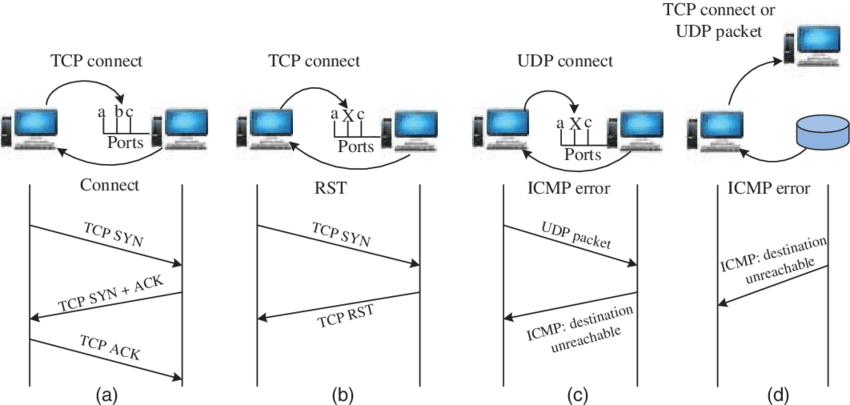
\includegraphics[scale=0.5]{figuras/tcp_connection_scheme.png}
    \caption{Esquema de estabelecimendo de conexões TCP e UDP (figura retirada de \cite{tcpudpscans}) \label{fig:tcpudp}}
    \subcaption{Conexão TCP bem sucedida}
    \subcaption{Conexão TCP mal sucedida: porta de destino fechada}
    \subcaption{Porta UDP de destino fechada}
    \subcaption{Endereço de IP de destino não existe}
\end{figure}



\section{Web Scraping e Web Crawling}

\textit{Web Scraping} é uma técnica de extração de dados de páginas \textit{web}. Ela geralmente é utilizada para extração de dados de sites de terceiros, onde não é viável a consulta de dados diretamente. 
\textit{Web Crawling} consistem em, recursiva e programáticamente, navegar através de páginas \textit{web} utilizando um algoritmo de busca em largura, extraindo determinadas informações obtidas com \textit{web scraping}. Dentre essas informações obtidas, está uma lista de links para outras páginas, que serão adicionadas na fila de páginas a serem escaneadas caso se enquadrem em determinados critérios, geralmente definidos pelo tipo de aplicação dos outros dados das páginas.

O principal uso conhecido dos \textit{web crawlers} é nos motores de busca (como DuckDuckGo ou Google), onde são extraidos \textit{links}, imagens e outras informações relevantes das páginas para consulta do público geral. No entanto, existem diversos outros casos de uso para tais ferramentas, já que é possível programá-las para extrair quaisquer informações disponíveis nas páginas. 

\section{SQL Injection}

A linguagem SQL (Structured Query Language ou Linguagem de Consulta Estruturada) é o principal método de interação com sistemas gerenciadores de bancos de dados relacionais (SGBDs), e por conta disso é utilizada em uma grande porcentagem dos serviços em produção. No entanto, quando os dados de entrada dos usuário não são propriamente sanitizados, é possível que eles contenham caracteres que influenciem a comunicação da aplicação com o SGBD. Caso o usuário seja mal intencionado, ele pode ser capaz de executar seus pŕoprios comandos SQL, o que determina se um sistema está vulnerável a \textit{SQL Injection}. 

Logo, \textit{SQL Injection} se trata de uma vulnerabilidade de execução de código remoto (RCE), que pode comprometer todos os dados da aplicação, ou até mesmo todo o sistema que a roda. 

Existem diversas maneiras de se evitar este tipo de vulnerabilidade, e geralmente não são difíceis de ser implementadas. Por exemplo, sanitizar as entradas dos usuários já torna essa vulnerabilidade muito mais difícil de acontecer (embora ainda possível, caso haja algum problema no método de sanitização). Da mesma forma, existem diversas maneiras com que uma vulnerabilidade de \textit{SQL Injection} pode ser explorada, como pode ser visto em mais detalhes na implementação do módulo de SQLMap do VuMoS \ref{item:sqlmap}, uma ferramenta que as detecta e explora.  